\documentclass[12pt,a4paper]{article}
\usepackage{mathtools}
\usepackage{parskip}
\usepackage[colorlinks=true, urlcolor=blue]{hyperref}
\usepackage{amsmath}
\usepackage{amssymb}
\usepackage{float}
\usepackage{fontenc}
\usepackage{graphicx}
\usepackage{caption}
\usepackage{subcaption}

\renewcommand\thesubsection{\thesection.\arabic{subsection}}
\renewcommand\thesubsubsection{\thesubsection.\alph{subsubsection}}

\newcommand{\tab}{\hspace*{2em}}

\title{ADNI Progress report}
\author{Devendra Goyal\\Uniqname: devendra}

\date{\today}

\begin{document}
\maketitle

\section{Statistics about the Data}
\label{sec:stats}

The results shown in this document are based on the ADNI-1
cohort. There are several pros and cons of this decision:

\subsection{Pros}

\begin{itemize}
\item All the pre-processed features uploaded on the ADNI website
  operate on the entire cohort, thus there is homogeneity in terms of
  the features available for each patient across each modailty. MRI
  images for ADNI-GO/2 have been processed using different versions of
  the same software, and are also collected using a higher resolution
  MRI machine. While this is not a dealbreaker per se, it will require
  significantly more work to process all the images using the same
  software and generate similar features.
\item Most of the recent literature (~5 years) relies on data from ADNI1
  only to report results. This will give us a chance to compare our
  results directly with some of these reported results.
\item ADNI-1 is the best dataset to track patients longitudinally, as
  it was started in $2004$ and we have about $8$ years' worth of data
  for all MCI and AD patients that the protocol chose to follow (more
  on this later). 
\end{itemize}

\subsection{Cons}

\begin{itemize}
\item ADNI1 has CSF data available for only about 20\% of the
  patients. This number will become even smaller when we look at the
  number of patients that have data available for all 3 modalities.
\end{itemize}

Below is a chart summarizing the study design:

\begin{figure}[ht]
  \centering
  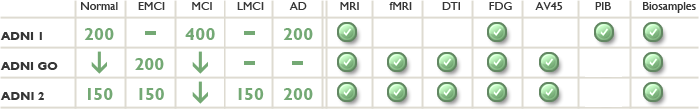
\includegraphics[width=\textwidth]{study-design.png}
  \caption{\label{fig:design}ADNI study design}
\end{figure}

The table below summarizes the number for the \textbf{ADNI1} cohort
only, for the MRI and PET modalities.

\end{document}